% IEEE standard conference template; to be used with:
%   spconf.sty  - LaTeX style file, and
%   IEEEbib.bst - IEEE bibliography style file.
% --------------------------------------------------------------------------

\documentclass[letterpaper]{article}
\usepackage{spconf,amsmath,amssymb,graphicx,svg}
\usepackage{todonotes}
\usepackage{fancyvrb}

% Example definitions.
% --------------------
% nice symbols for real and complex numbers
\newcommand{\R}[0]{\mathbb{R}}
\newcommand{\C}[0]{\mathbb{C}}

% bold paragraph titles
\newcommand{\mypar}[1]{{\bf #1.}}

% Title.
% ------
\title{Implementation of an optimized authenticated encryption scheme}
%
% Single address.
% ---------------
\name{Alessandro Giaconia, Diana Khimey, Filippo Visconti, Lorenzo Paleari}
\address{Department of Computer Science\\ ETH Z\"urich\\Z\"urich, Switzerland}


\begin{document}
%\ninept
%
\maketitle
%

% The hard page limit is 6 pages in this style. Do not reduce font size
% or use other tricks to squeeze. This pdf is formatted in the American letter format, so the spacing may look a bit strange when printed out.

\begin{abstract}
	This paper presents the optimization performed on an authenticated encryption scheme, ChaCha20 for encryption and Blake3 for authentication. The focus is on enhancing performance through vectorization and parallelization, addressing the challenges of processing large data efficiently. Our results demonstrate significant improvements in throughput and efficiency, making our scheme highly suitable for modern high-performance applications that demand robust security and data integrity. The paper contributes an open-source implementation and offers insights into the scalability and performance of authentication and encryption in multi-core environments.
\end{abstract}

\section{Introduction}\label{sec:intro}

% Do not start the introduction with the abstract or a slightly modified
% version. It follows a possible structure of the introduction.
% Note that the structure can be modified, but the
% content should be the same. Introduction and abstract should fill at most the first page, better less.

\mypar{Motivation}
% The first task is to motivate what you do.  You can
% start general and zoom in one the specific problem you consider.  In
% the process you should have explained to the reader: what you are doing,
% why you are doing, why it is important (order is usually reversed).
%
% For example, if my result is the fastest sorting implementation ever, one
% could roughly go as follows. First explain why sorting is important
% (used everywhere with a few examples) and why performance matters (large datasets,
% realtime). Then explain that fast implementations are very hard and
% expensive to get (memory hierarchy, vector, parallel).
%
% Now you state what you do in this paper. In our example:
% presenting a sorting implementation that is
% faster for some sizes as all the other ones.
In an era characterized by the exponential growth of data and the escalating prevalence of digital communication, safeguarding sensitive information has become an indispensable priority. The continuous evolution of technology introduces new challenges in upholding the confidentiality and integrity of data exchanged over networks.

This project embarks on a journey focused on implementing a state-of-the-art, optimized, high-performance authenticated encryption scheme. The motivation driving this initiative arises from the necessity for robust cryptographic solutions that not only ensure security but also exhibit efficient runtimes. Authenticated encryption schemes serve as fundamental pillars in modern cryptography, offering a comprehensive solution for ensuring confidentiality, integrity, and authenticity of data. 
These schemes find wide-spread application in various contexts, including TLS, SSH, IPsec, and numerous others.

%It is essential to note that the key distinction between authenticated encryption schemes and traditional encryption schemes lies in the former's ability to not only ensure confidentiality but also provide data integrity and authenticity, addressing the comprehensive security needs of modern applications.

Given that authenticated encryption schemes are nowadays used in many critical applications, it is extremely important to provide the best performance possible, and it is necessary to avoid being limited by factors like file size.

For these reasons, our project leverages the strengths of ChaCha20 and Blake3, prioritizing efficiency and speed, and being targeted toward the most difficult cases, namely instances dealing with huge files.

\mypar{Related work}

A significant study by R. Velea et al. \cite{parallelchacha} delves into the performance implications of parallelizing the ChaCha20 encryption cipher across multi-core CPUs and GPUs. The research, conducted using the serial implementation from the BoringSSL encryption library and accelerated through OpenMP and OpenCL, provides valuable insights into the efficiency gains achieved by parallelization. The study particularly highlights the reduction in power consumption with a parallel implementation, showcasing its impact on resource utilization.

It is worth noting that, currently, there is a distinct lack of open-source implementations focusing on the parallel aspects of ChaCha20. Our work aims to contribute to this field by providing an open-source parallel implementation of ChaCha20, addressing the existing gap in the availability of such resources.

For our Blake implementations, we followed closely the algorithm description provided in the original paper \cite{blake}. As a reference, we also used the single-threaded implementation provided by the paper's authors \cite{gitblake}.
\section{Background}\label{sec:background}
In this section, we give a brief overview of the background necessary to understand the rest of the report.
In particular, we introduce the concepts of encryption and authentication, and we explain the algorithms we use.
% Give a short, self-contained summary of necessary
% background information. For example, assume you present an
% implementation of sorting algorithms. You could organize into sorting
% definition, algorithms considered, and asymptotic runtime statements. The goal of the
% background section is to make the paper self-contained for an audience
% as large as possible. As in every section
% you start with a very brief overview of the section. Here it could be as follows: In this section
% we formally define the sorting problem we consider and introduce the algorithms we use
% including a cost analysis.

\mypar{Encryption}
Encryption is a fundamental concept in information security that involves converting plaintext data into a secure and unreadable form, referred to as ciphertext. The primary goal of encryption is to protect sensitive information from unauthorized access or tampering during transmission or storage. This process ensures that only authorized parties with the appropriate decryption key can access and decipher the original data.

\mypar{ChaCha20}
ChaCha20, detailed in \cite{chacha20}, serves as a symmetric key stream cipher with the dual purpose of ensuring data confidentiality and integrity. Recognized for its simplicity, speed, and resistance to cryptographic attacks, it proves to be an excellent fit for this project due to its high parallelizability.

The functioning of the ChaCha20 algorithm involves taking a key, a nonce and a counter and subjecting them to a series of additions, rotations, and XOR operations. This process produces a keystream that is then XORed with the plaintext. These operations facilitate swift computation even on general-purpose hardware without specific instruction sets like AES-NI.

Today, ChaCha20 is widely used in various security protocols and applications, including TLS (Transport Layer Security) for secure communication on the internet. Notably, in TLS v1.3, it stands as the only alternative to the Advanced Encryption Standard (AES). This attests to its reliability and versatility in secure communication, highlighting its important role in today's cryptographic systems.

\mypar{Authentication}
Authentication is the process through which the integrity and origin of data are verified, to ensure that it remains untampered and confirming that it originated from the expected sender. %This verification process holds significant importance in diverse fields, including secure communication, electronic commerce, and various other domains.

To achieve authentication, Message Authentication Code (MAC) is commonly employed. A MAC is a concise piece of information utilized to authenticate a message, working in conjunction with a secret key. The recipient of the message can validate its authenticity by recalculating the MAC and comparing it with the original MAC. This mechanism provides a secure means of ensuring that the received data has not been altered and originates from the expected source.

% As an aside, don't talk about "the complexity of the algorithm.'' It's incorrect,
% problems have a complexity, not algorithms.
\mypar{Blake3}
We opted for Blake3 as the authentication component of our scheme, driven by its notable combination of high performance and robust security guarantees. Blake3 is inherently parallelizable, enhancing its suitability for our implementation. The implementation, carried out in the C language, employs two distinct approaches: one utilizing a stack for versatility, and the other employing a more efficient divide-and-conquer strategy, albeit with slightly reduced flexibility, but significantly improved performance.

%Blake3 operates as a cryptographic hash function with a built-in MAC function, the specific feature we are leveraging.
At a high level, Blake3 processes input by dividing it into chunks of up to 1024 bytes and arranges them as the leaves of a binary tree. These chunks are then compressed using a compression function, conducting a series of operations on the input and producing a 64-byte output, the chaining value. The chaining value from each chunk becomes the input for the subsequent chunk, this process continues until all chunks are processed. The chunks effectively represent the leaves of a binary tree, and the tree is traversed from the bottom up. At each level, the chaining values of two children nodes are combined until reaching the root node. The final result is the chaining value of the root node, obtained through iterations of this process.

To obtain an output of arbitrary length, the last call to the compression function can be repeated with an increased counter, ensuring adaptability to various application requirements.

\section{Our Proposed Method}\label{sec:yourmethod}
In this section, we dive into the details of our implementation. We describe how we implemented the algorithms,
and we explain the optimizations we used to achieve high performance.
% Now comes the ``beef'' of the report, where you explain what you
% did. Again, organize it in paragraphs with titles. As in every section
% you start with a very brief overview of the section.
%
% In this section, structure is very important so one can follow the technical content.
%

\mypar{ChaCha20}
Our implementation of ChaCha20 aligns with the specifications outlined in the RFC \cite{rfcchacha}. The algorithm involves processing a 64-bytes stream through a block function, where a fixed number of XORs, rotations, and additions are performed. Although the algorithm itself offers limited room for improvement due to its inherent simplicity, we pursued optimizations for single-core performance. 

We began our optimization efforts with fundamental techniques, like inlining, which, to our surprise, proved more effective than using macros. We also delved into improving memory usage efficiency. However, these initial steps did not achieve the desired level of efficiency.

To further enhance performance, we performed vectorisation, specifically employing AVX-256 to optimize the block function. This proved to be a significant improvement, showcasing the algorithm's responsiveness to advanced optimization strategies.

We later moved into the parallel implementation, which leveraged the OpenMP library. Taking advantage of the independence of each block, parallelization required minimal modifications to the existing algorithm. However, optimizing for cache spatial locality demanded experimentation with various OpenMP scheduling options, adding an extra layer of complexity to the fine-tuning process.
We experimented with all different scheduling options, namely: static, dynamic, and guided. In the static approach, the iteration space is divided into chunks of approximately equal size, with at most one chunk assigned to each thread. Dynamic, on the other hand, assigns a loop iteration (or a user-defined chunk) to each thread. When a thread finishes its assigned task, it requests a new one. Guided operates similarly to Dynamic but begins by assigning larger chunks and progressively reduces the dimension until reaching 1.

\mypar{Blake3}
In this subsection, we describe our implementations of the Blake3 algorithm, which are based on and closely follow the original Blake3 paper that describes the algorithm in detail \cite{blake}.
Given their different strengths and characteristics, we also included a dispatcher that chooses the best implementation based on the input size, to always guarantee a correct output.

\mypar{Divide-and-conquer version}
\begin{figure}[h]
	\begin{center}
		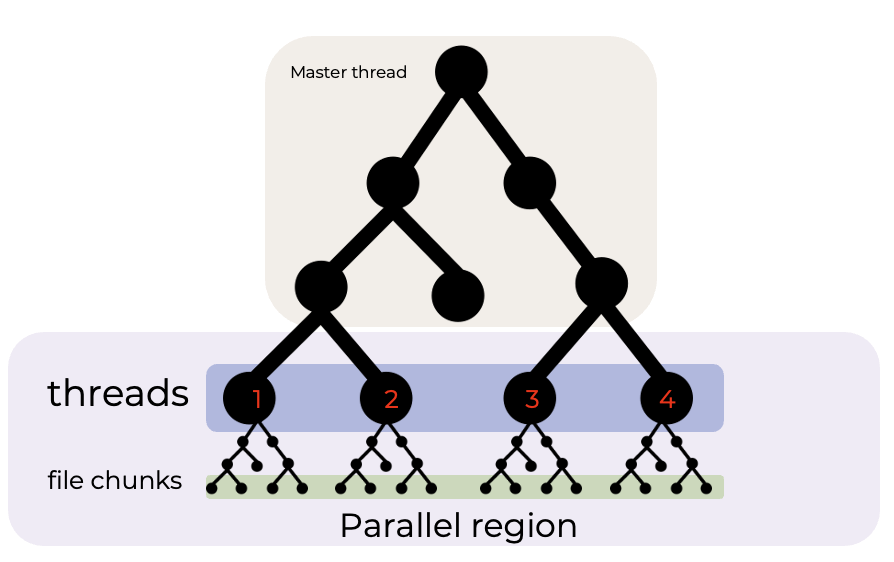
\includegraphics[width=0.45\textwidth]{figures/div_conq.png}
	\end{center}
	\caption{High-level visualization of the divide and conquer approach}\label{fig:divide_and_conquer}
\end{figure}
The divide-and-conquer version of the algorithm, also referred as Full Tree version, relies on the premise that the entire input is accessible at the outset of the computation. This enables an equitable distribution of work among multiple threads, each operating on distinct portions of the input, and subsequently eliminating dependencies among them. The threads function concurrently until they reach the base case, wherein each thread is left with one node.

Upon reaching this base case, the threads transmit their individual results to the parent thread, which consolidates these outcomes and returns the final result. This parallelized approach enhances the algorithm's efficiency, leveraging the availability of the complete input early in the computation to facilitate concurrent and independent processing by multiple threads.

To facilitate parallelization in our algorithm, we leverage the Open-MP library, streamlining the process of distributing computation across threads once a parallel region is established. Additionally, we enhance performance by vectorizing the compression function, the most computationally intensive component of the algorithm, using 128bit vector instructions by partially adopting code from the reference implementation \cite{gitblake}.

The primary advantage of this approach lies in its scalability, attributed to the even distribution of work among threads with no inter-thread dependencies. This characteristic allows us to achieve commendable speedups, as detailed in the results section. However, it is important to note that this approach, while highly scalable, has limitations in flexibility. Specifically, it necessitates the availability of the entire input at the commencement of the computation (which aligns with our requirements) and is most effective when the input conforms to a full binary tree structure. 
% These considerations, although relevant, are mitigated by the suitability of our use case.

\mypar{Stack version}
\begin{figure}[h]
	\begin{center}
		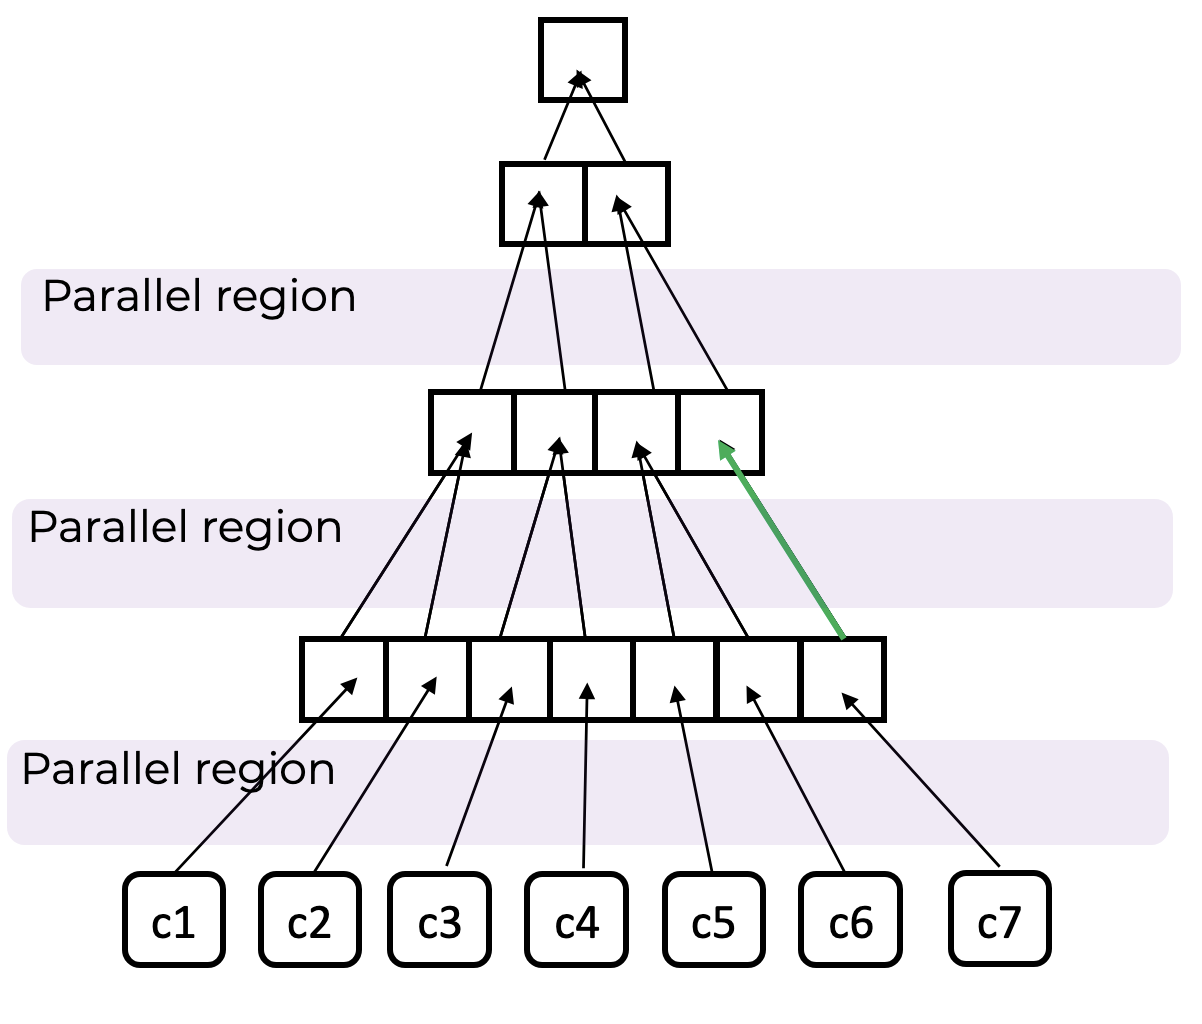
\includegraphics[width=0.34\textwidth]{figures/stack_method.png}
	\end{center}
	\caption{High-level visualization of the parallel stack approach}
 \label{fig:stack-exp}
\end{figure}

As opposed to the Full Tree algorithm described above, this approach uses a stack to track the progress of parent and child chunks up to the root node. Instead of splitting the entire tree across threads, this algorithm parallelizes the compressions between different levels of the tree. Each thread can then access the chaining values of the child nodes stored on the stack, and store the result of the compression. To prevent false sharing and ensure proper workload distribution, each thread reads and writes from and to unique locations on the stack. As in the divide-and-conquer approach, parallelization is achieved through the use of the Open-MP library and by further performance improvements are achieved by vectorizing the compression function.

The primary benefit of this approach is that it simplifies the logic of compressing files that do not create a full binary tree. It does this by leveraging the stack, and continuously pushing single child chunks up the tree, as is highlighted by the green arrow in Fig. \ref{fig:stack-exp}. However, it forces threads to continuously switch between parallel and sequential regions, such that the stack is synchronized between each tree level. These transitions cause significant overhead in this approach compared to the divide-and-conquer algorithm, but overall leads to simpler logic when dealing with imperfect file sizes.

\section{Experimental Results}\label{sec:exp}

% Here you evaluate your work using experiments. You start again with a
% very short summary of the section. The typical structure follows.
Both encryption and authentication were tested on different versions to better detect implementation bottlenecks, initially working on single core and later improving the parallelization of the code to reach better speed up due to the multi-core environment.
Every implementation has been tested with input size varying from 1MB to 128GB scaling with a factor of 2. This goes from small dimensions that fits perfectly inside the cache to huge dimensions, while still ensuring that the computation fits the available RAM.

\mypar{Experimental setup}
Our experiments were conducted on the Ault Cluster of the Swiss National Supercomputing Centre (CSCS). We specifically utilized a node with the following specifications:\vspace{2pt}
\begin{itemize}
  \item \textbf{Processors}: 2x AMD EPYC 7742 64 cores @ 2.25 GHz.
  \item \textbf{Memory}: 256GB of RAM for each processor. 512GB Total. We tested RAM memory bandwidth using the STREAM benchmark\cite{stream}, it showed a maximum of 130GB/s on a single processor and 270GB/s across the full node (see Appendix for full benchmark results \ref{sec:A}\ref{subsec:A1}).
    \item \textbf{L3 Cache}: Each AMD EPYC 7742 processor features a 256MB L3 cache, segmented into 16 blocks of 16MB each.
    % \item \textbf{Physical Dies}: The processor comprises 9 dies - 8 Core Complex Dies (CCDs) for processing and 1 IO die\cite{Epyc_rome}. Each CCD is comprised of 8 cores distributed across two CPU Complexes (CCXs), with each CCX containing 4 cores and sharing a physical L3 cache (16MB)\cite{memory_structure}. Notably, CCXs on the same die do not have direct cache access to each other, necessitating communication through the IO die. This architecture can lead to significant NUMA effects, especially when sharing data across cores in different CCXs\cite{amd_mem_barrier}.
    \item \textbf{NUMA Configuration}: The node's dual-socket setup forms two NUMA (Non-Uniform Memory Access) regions, each with one processor and 256GB of RAM.
\end{itemize}

Compiler, version and used flags vary between authentication and encryption algorithms and were carefully chosen to achieve the best performance possible. In particular, some flags were taken from AMD's specialized guide on the EPYC 7002 processor family \cite{amd}.
\begin{itemize}
    \item \textbf{Blake}: \texttt{gcc 10.3.0}, \texttt{ -O3 -march=native}
    %\item \textbf{ChaCha20 - NV}: \texttt{gcc 8.4.1}, \texttt{ -O3 -ffast-math -march=znver1 -mtune=znver1 -fopenmp -mfma -mavx2}
    \item \textbf{ChaCha20}: \texttt{gcc 13.2.0}, \texttt{ -O2 -ffast-math -march=znver2 -mtune=znver2 -fopenmp -mfma -mavx2 -fprefetch-loop-arrays \\-param prefetch-latency=300}
\end{itemize}

%\mypar{Results}
%In this section, we will show and discuss the results obtained through %our experiments.

%\todo[inline]{To change or remove}
% Next divide the experiments into classes, one paragraph for each. In each class of experiments you typically pursue one questions that then is answered by a suitable plot or plots. For example, first you may want to investigate the performance behavior with changing input size, then how your code compares to external benchmarks.
\begin{figure}
\centering
	\includesvg[width=\columnwidth]{figures/enc_tp_single.svg}
	\caption{Comparison of performance over changing input sizes of the single-threaded versions of our implementations and the reference implementation. Higher is faster.
  \label{fig:enc_single_thread}}
  \vspace{-4pt}
\end{figure}

\mypar{ChaCha20 - Single-threaded comparison}
%In this section we want to fix a starting point from which we are going to make parallelization further on, we also want to put our code in comparison with other state-of-the-art solutions and see how well we perform.
Figure \ref{fig:enc_single_thread} showcases our single-threaded implementation's performance, comparing it to the \texttt{libsodium} library, one of the fastest crypto-libraries available.

Our results demonstrate a highly efficient vectorized single-core implementation that achieves a throughput of 2.32 GB/s improving of a factor of 5.30x the base version that sits at just 0.44GB/s.

Furthermore our vectorized implementation exhibits such efficiency to even surpass \texttt{libsodium} with a factor of 1.25x.
Lastly we can observe, throughout all the input sizes, the throughput consistency showing an absence of performance degradation with bigger inputs.

\begin{figure}
\centering
	\includesvg[width=\columnwidth]{figures/comparison_bar_graph.svg}
	\caption{Comparison of different OpenMP scheduling. Values represent the Throughput using 128 threads with the vectorized version of the code. Higher is faster.
  \label{fig:enc_comparison}}
  \vspace{-5pt}
\end{figure}

\mypar{ChaCha20 - Different scheduling}
Utilizing OpenMP to parallelize our vectorized code comes with a question, which of the scheduling policies, mentioned and described in the OpenMP manual \cite{openMP}, is the best. 

Figure \ref{fig:enc_comparison} illustrates our findings, indicating that static scheduling outperforms the others.
Our implementation encrypts input blocks independently using a fixed set of instructions, giving consistent encryption times per block. This behaviour benefits static scheduling, while dynamic and guided policies gives better results for tasks with variable processing times. 

\begin{figure}[h]
\centering
	\includesvg[width=\columnwidth]{figures/enc_tp_opt2.svg}
	\caption{Multi-threaded vectorization performance across varying input sizes. Between parenthesis the speedup achieved with an input size of 128GB. Higher is faster.
  \label{fig:enc_opt2}}
  \vspace{-5pt}
\end{figure}

\mypar{ChaCha20 - Final results}
Lastly, we want to understand the limits of our best ChaCha20 implementation, pushing it to its limits by testing it against the full 128 core of the node.
We now analyse and understand the results showed by Figure \ref{fig:enc_opt2} in particular we concentrate on three interesting behaviours.

The initial observation in our study is the pattern of speedup (indicated in the graph legend within parentheses) for input sizes measured in GBs. Performance scale perfectly up until 16 Threads, reaching a sudden stop at a speedup of ~28x when testing on 32 and 64 Threads and lastly, it gets to 55x when using 128 Threads.
Given that the node consists of two CPUs, each with 64 cores, the increase in speedup when moving from 64 to 128 threads can be attributed to the utilization of both CPUs. This observation also suggests an absence of noticeable NUMA effects in this scenario. This can be explained by our ChaCha20 implementation: each block of input to be encrypted operates independently, allowing OpenMP to efficiently manage thread scheduling and data distribution across the two NUMA regions, therefore avoiding performance bottleneck.
The observed pause in speedup at ~28x can be explained using the results of our memory bandwidth benchmark. When using 64 cores, the maximum achievable memory bandwidth (MemBW) is 138GB/s. This number becomes significant when compared to the 65.7GB/s throughput achieved by our implementation at 64 cores. Considering the need to read, encrypt, and write back the input, the data transfer between RAM and CPU amounts to at least 131.4GB/s. This result come close the maximum bandwidth capacity. The slight discrepancy between these numbers can be attributed to difference in compilers, flags, and code, leading to the conclusion that we have likely reached the maximum available bandwidth.

Another noticeable anomaly consist in the huge throughput reached by 64 and 128 Threads with inputs ranging in the hundreds of MBs. New random inputs are generated each run, which are going to fit in last level cache if their dimension is less than 256/512MB (1 or 2 CPUs). This allows the processor to leverage the full MemBW just to write back the input. Indeed results show double the throughput reaching 240GB/s. Regrettably, as soon as we try to encrypt bigger data we will not fit in cache resulting in being constrained to half the throughput as explained before.

Lastly, we noticed a consistency difference between large (GB-sized) and smaller input sizes. Larger inputs take longer to compute ensuring consistent runtimes. On the other hand, smaller inputs take much shorter time to compute, in the order of few $\mu$s and thus even the slightest change in runtimes shows bigger inconsistency in the graph.


\mypar{Blake - Single-threaded comparison}
Through Figure \ref{fig:singleblake}, we will analyze how our implementations (\texttt{blake\_f} represents the full-tree version, while \texttt{blake\_d} represents the stack version) compare to the reference implementation (\texttt{blake\_ref}), written in C by the authors of the original paper.

From the graph, the performance of our stack implementation closely follows the reference one, since the original approach also uses a stack. The full-tree version is slightly penalized by the overhead it introduces for very small inputs. However, on inputs larger than 4-16MB, it does achieve a better throughput. The increase in performance sits stably at around 16\%.

\begin{figure}[h]
\centering
	\includesvg[width=\columnwidth]{figures/single_plot_cumulative.svg}
	\caption{Comparison of performance over changing input sizes of the single-threaded versions of our implementations and the reference implementation. Higher is faster.
  \label{fig:singleblake}}
  \vspace{-5pt}
\end{figure}

\mypar{Blake - Stack}
\begin{figure}[h]
	\begin{center}
		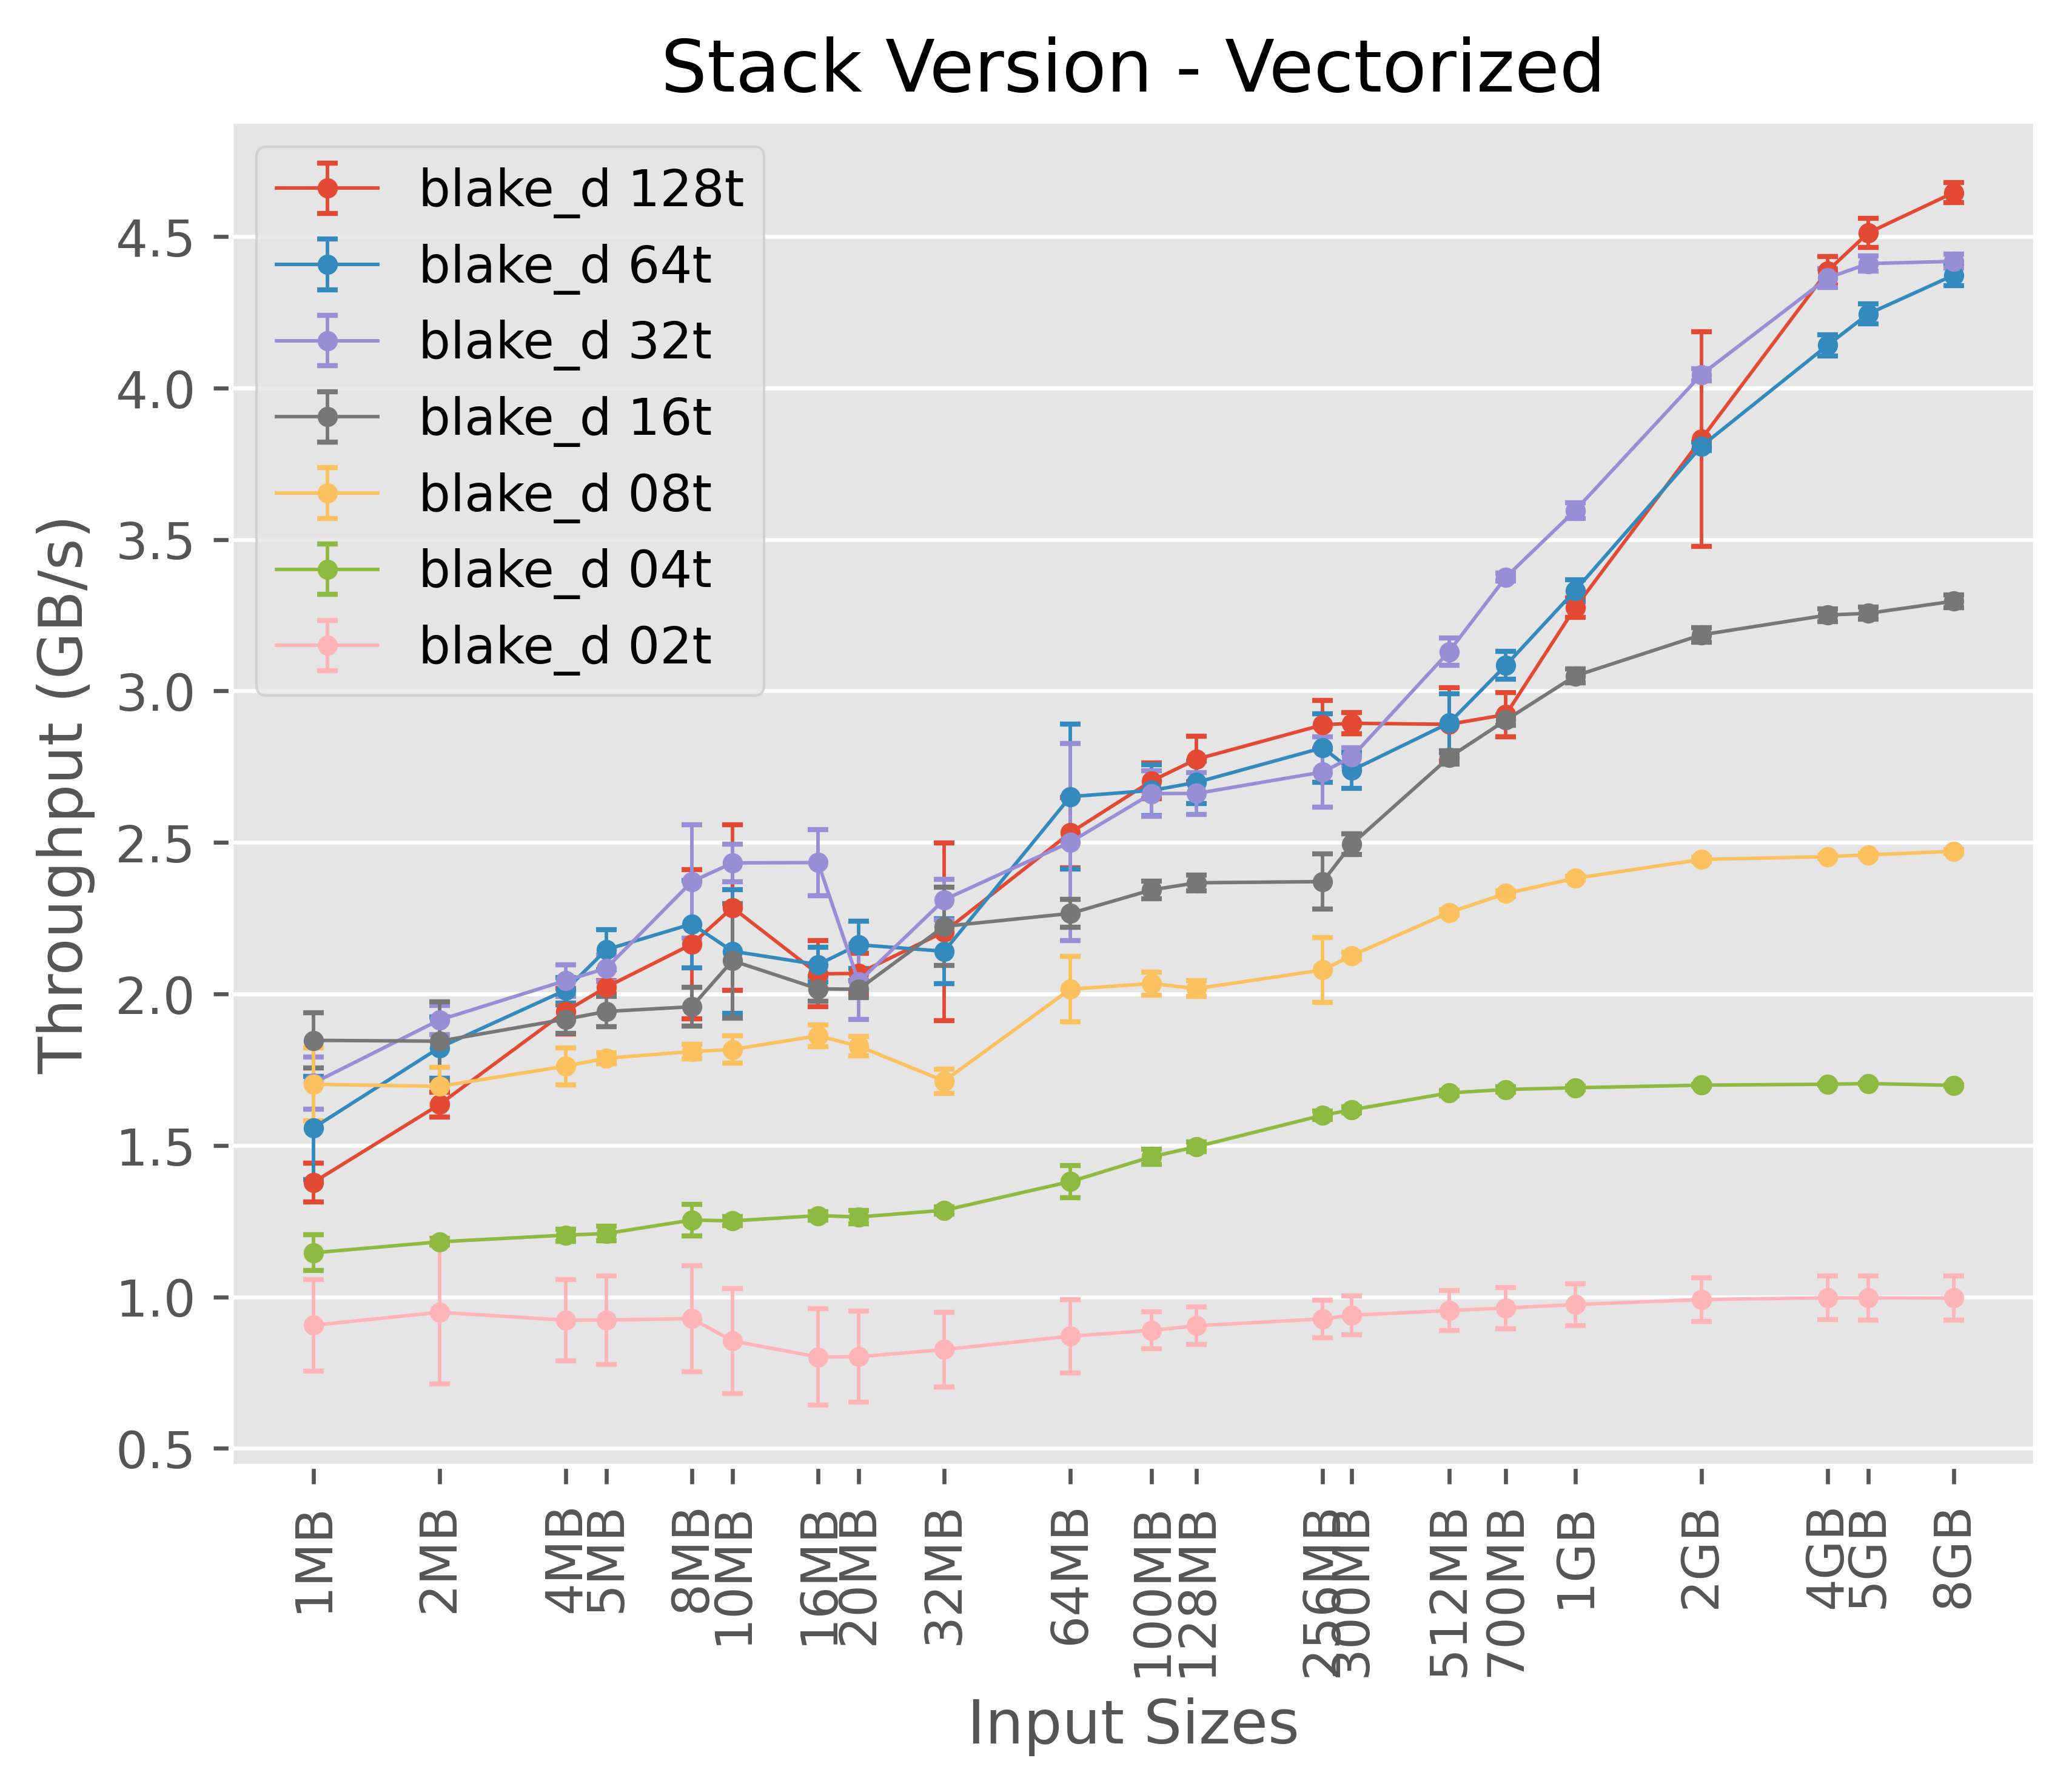
\includegraphics[width=0.45\textwidth]{figures/stack_vec_plot.png}
	\end{center}
	\caption{Performance for growing input sizes of the parallelized and vectorized version of the stack approach. Speedup is shown for an increasing number of threads.}
 \label{fig:stack-multithread}
 \vspace{-5pt}
\end{figure}
In Fig. \ref{fig:stack-multithread}, we show the performance of the parallelized stack implementation for an increasing number of cores and input sizes. 

The throughput performance scales roughly linearly to the number of threads, when the number of cores is below 32. However, as can be observed, speedups are negligible for a larger number of cores. This is likely due to the overhead of continuously creating and synchronizing a larger number of threads.

\mypar{Blake - Full Tree}
% For some tips on benchmarking including how to create a decent viewgraph see pages 22--27 in \cite{Pueschel:10}.
In Figure \ref{fig:fulltreeblake}, we aim to analyze how our fastest implementation scales with the number of cores.


\begin{figure}[h]
\centering
	\includesvg[width=\columnwidth]{figures/vec_plot_cumulative_f.svg}
	\caption{Performance over changing input sizes of the multi-threaded, vectorized version of the divide-and-conquer implementation. Higher is faster.
  \label{fig:fulltreeblake}}
  \vspace{-5pt}
\end{figure}

As it is possible to observe, there is a consistent increase of performance up until reaching 64 cores, which sees the throughput double as the number of cores doubles as well. However, going from 64 to 128 cores, the improvement is smaller, and the throughput fluctuates a bit. This is due to the fact that the machine has 2 64-core CPUs, and using both of them for the same program results in some overhead, likely due to slower memory accesses.

We achieved a maximum throughput of 39-50 GB/s, which, converted into bytes per cycle for reference, are equivalent to 18-23 B/C.

In the future, this issue could be fixed by changing the logic of the program in order to implement a multi-process computation, and spawning two different processes, task-setting them on one CPU each, such that we can have a finer control over memory traffic.

As a sanity check, we also bench-marked our code with the compression function disabled (the function body was emptied). This led to a final, ideal throughput of 120 GB/s for the 128 thread Full Tree Version.


% {\bf Comments:}
% \begin{itemize}
% 	\item Every plot answers a question. You state this question and extract the
% 	      answer from the plot in its discussion.
% 	\item Every plot should be referenced and discussed.
% \end{itemize}

\section{Conclusions}
This study introduced a comprehensive exploration into optimizing authenticated encryption through the implementation and enhancement of ChaCha20 and Blake3 algorithms.

The ChaCha20 single-threaded comparison displayed a highly efficient implementation, surpassing the \texttt{libsodium} library with a notable 1.25x speedup. The parallel version showcased exceptional scalability, achieving a peak throughput of 130 GB/s with linear speedups observed from 1 to 32 threads ultimately reaching the limit imposed by the CPU memory bandwidth. These results provide compelling evidence of the overall efficiency of our implementations.

In the realm of Blake3, we achieved single-thread performance comparable to that of the reference implementation. The multi-threaded stack approach to the algorithm demonstrates a substantial improvement in performance compared to the reference implementation, even while using the same stack structure to manage compression. The divide-and-conquer approach was shown to scale virtually indefinitely with the number of cores, indicating promising potential for uses with massive file sizes.

\mypar{Future Work}
The project lays the foundation for future enhancements and explorations. For ChaCha20, further investigations into alternative vectorization strategies and the utilization of advanced instruction sets (AVX-512) could yield additional performance improvements. Testing on newer architecture can also benefit the research and showcase the full scalability of our implementation without being limited by the memory bandwidth. 

In the case of Blake3, scalability on systems with multiple CPUs are areas worth exploring. For further improvements, it would be interesting to explore how the encryption problems can be divided in order to take advantage of the stack version's simple logic as well as the scalability of the divide-and-conquer approach. Just as for ChaCha20, the use of vectorization strategies such as AVX-512 could lead to even further performance improvements for Blake3.

Moreover, a comprehensive security analysis of the implemented scheme is essential to ensure its robustness against potential vulnerabilities - such as side channel attacks. 

% References should be produced using the bibtex program from suitable
% BiBTeX files (here: bibl_conf). The IEEEbib.bst bibliography
% style file from IEEE produces unsorted bibliography list.
% -------------------------------------------------------------------------
\bibliographystyle{IEEEbib}
\bibliography{bibl_conf}

\newpage
\renewcommand{\thesection}{\Alph{section}}
\renewcommand{\thesubsection}{\arabic{subsection}}
\setcounter{section}{0}
\section{Appendix}
\label{sec:A}
\subsection{Benchmarks}
\label{subsec:A1}
\textbf{Single processor memory bandwidth}
{\tiny
\begin{verbatim}
-------------------------------------------------------------
STREAM version $Revision: 5.10 $
-------------------------------------------------------------
This system uses 4 bytes per array element.
-------------------------------------------------------------
Array size = 3000000000 (elements), Offset = 0 (elements)
Memory per array = 11444.1 MiB (= 11.2 GiB).
Total memory required = 34332.3 MiB (= 33.5 GiB).
Each kernel will be executed 100 times.
 The *best* time for each kernel (excluding the first iteration)
 will be used to compute the reported bandwidth.
-------------------------------------------------------------
Number of Threads requested = 64
Number of Threads counted = 64
-------------------------------------------------------------
Your clock granularity/precision appears to be 1 microseconds.
Each test below will take on the order of 178468 microseconds.
   (= 178468 clock ticks)
Increase the size of the arrays if this shows that
you are not getting at least 20 clock ticks per test.
-------------------------------------------------------------
WARNING -- The above is only a rough guideline.
For best results, please be sure you know the
precision of your system timer.
-------------------------------------------------------------
Function    Best Rate MB/s  Avg time     Min time     Max time
Copy:          141867.4     0.169484     0.169172     0.169902
Scale:         142325.9     0.168982     0.168627     0.169334
Add:           143459.4     0.251262     0.250942     0.251731
Triad:         143444.0     0.251348     0.250969     0.251694
-------------------------------------------------------------
Solution Validates: avg error less than 1.000000e-06 on all three arrays
-------------------------------------------------------------
\end{verbatim}
}
\textbf{Full node memory bandwidth}
{\tiny
\begin{verbatim}
-------------------------------------------------------------
STREAM version $Revision: 5.10 $
-------------------------------------------------------------
This system uses 4 bytes per array element.
-------------------------------------------------------------
Array size = 3000000000 (elements), Offset = 0 (elements)
Memory per array = 11444.1 MiB (= 11.2 GiB).
Total memory required = 34332.3 MiB (= 33.5 GiB).
Each kernel will be executed 100 times.
 The *best* time for each kernel (excluding the first iteration)
 will be used to compute the reported bandwidth.
-------------------------------------------------------------
Number of Threads requested = 128
Number of Threads counted = 128
-------------------------------------------------------------
Your clock granularity/precision appears to be 1 microseconds.
Each test below will take on the order of 83415 microseconds.
   (= 83415 clock ticks)
Increase the size of the arrays if this shows that
you are not getting at least 20 clock ticks per test.
-------------------------------------------------------------
WARNING -- The above is only a rough guideline.
For best results, please be sure you know the
precision of your system timer.
-------------------------------------------------------------
Function    Best Rate MB/s  Avg time     Min time     Max time
Copy:          283249.0     0.084882     0.084731     0.085087
Scale:         284431.1     0.084562     0.084379     0.084783
Add:           286635.4     0.125829     0.125595     0.126814
Triad:         286662.6     0.125799     0.125583     0.126066
-------------------------------------------------------------
Solution Validates: avg error less than 1.000000e-06 on all three arrays
-------------------------------------------------------------
\end{verbatim}
}

\end{document}
